\section{JS ecosystem}\label{js-ecosystem}

\begin{quote}
as for 05.06.2017
\end{quote}

\begin{quote}
still work in progress
\end{quote}

\begin{quote}
main todos at the end
\end{quote}

\subsection{Introduction}\label{introduction}

The influential post
\href{https://hackernoon.com/how-it-feels-to-learn-javascript-in-2016-d3a717dd577f}{How
it feels to learn JavaScript in 2016} highlighted important feature of
JavaScript - a vast amount of JavaScript frameworks avaiable for
developers. But feelings are not enough to describe the whole ecosystem
and we need some data. Some of them were collected by
\href{http://stateofjs.com/}{the State of JavaScript Survey} where we
can find answers to questions on topics ranging from front-end
frameworks and state management, to build tools and testing libraries.
For those who are starting with web-development I would recommend to
read
\href{https://medium.freecodecamp.com/a-study-plan-to-cure-javascript-fatigue-8ad3a54f2eb1}{A
Study Plan To Cure JavaScript Fatigue}.

My personal goal here is to analyse the most popular frameworks to
highlight another troublesome feature of JavaScript. There is not only
vast amount of the frameworks, but also the vast amount of versions of
each framework. It is hard for the beginner to study particular
framework based on the materials and courses avaiable online, because
there are becoming outdated very quickly. Even though that for most of
them principles are not changing some features are
appearing/disappearing often. But not only frameworks are changing. All
existing JavaScript labels can give you a headache. The first encouter
of ES5, ES6 and ES2016 can be frightening, and the advice that you can
learn babel to resolve the problem is not helping. For those who are not
familiar with them - here you have nice blog post about
\href{https://benmccormick.org/2015/09/14/es5-es6-es2016-es-next-whats-going-on-with-javascript-versioning/}{JavaScript
versioning}.

Based on github repos and npm stats I will check how often new version
of each framework is released with emphasis on the major releases. Based
on the \href{http://stateofjs.com/}{the State of JavaScript Survey} I
will focus on the following frameworks:

\begin{itemize}
\tightlist
\item
  Front-End \href{http://stateofjs.com/2016/frontend/}{survey}

  \begin{itemize}
  \tightlist
  \item
    \protect\hyperlink{react}{React} :white\_check\_mark:
  \item
    Angular :white\_check\_mark:
  \item
    Ember :white\_check\_mark:
  \item
    Vue :white\_check\_mark:
  \item
    Backbone :white\_check\_mark:
  \end{itemize}
\item
  State Management
  \href{http://stateofjs.com/2016/statemanagement/}{survey}

  \begin{itemize}
  \tightlist
  \item
    Redux :white\_check\_mark:
  \item
    Mobx
  \item
    Relay
  \end{itemize}
\item
  Full- Stack \href{http://stateofjs.com/2016/fullstack/}{survey}

  \begin{itemize}
  \tightlist
  \item
    Meteor :white\_check\_mark:
  \item
    FeathersJS
  \item
    DoneJS
  \end{itemize}
\item
  Build Tools \href{http://stateofjs.com/2016/buildtools/}{survey}

  \begin{itemize}
  \tightlist
  \item
    Webpack :white\_check\_mark:
  \item
    Grunt
  \item
    Gulp
  \item
    Browserify
  \end{itemize}
\item
  \protect\hyperlink{nodeJS}{Node.js} :white\_check\_mark:
\end{itemize}

The analysis is done with \href{https://www.r-project.org/}{R} and
presented using \href{https://pages.github.com/}{GitHub Pages}. All
codes are available on GitHub

\subsection{Motivation}\label{motivation}

Some part of my motivation was described in the introduction. However it
lacks data. Is it JavaScript really important? How important is it?

Using
\href{https://bigquery.cloud.google.com/dataset/httparchive:runs}{Google
BigQuery httparchive datasets} I check the growth rate of bytes count
for HTML and JS content. Starting from 2012-01-01 till 2017-04-01 the
average size of JS code for 10,000 most popular webpages grew by 200\%
while HTML content only by \textasciitilde{}50\%. It shows how important
JS is for the web development right now. Keep in mind that those data do
not show e.g.~the server-side JS implementations.

\begin{figure}
\centering
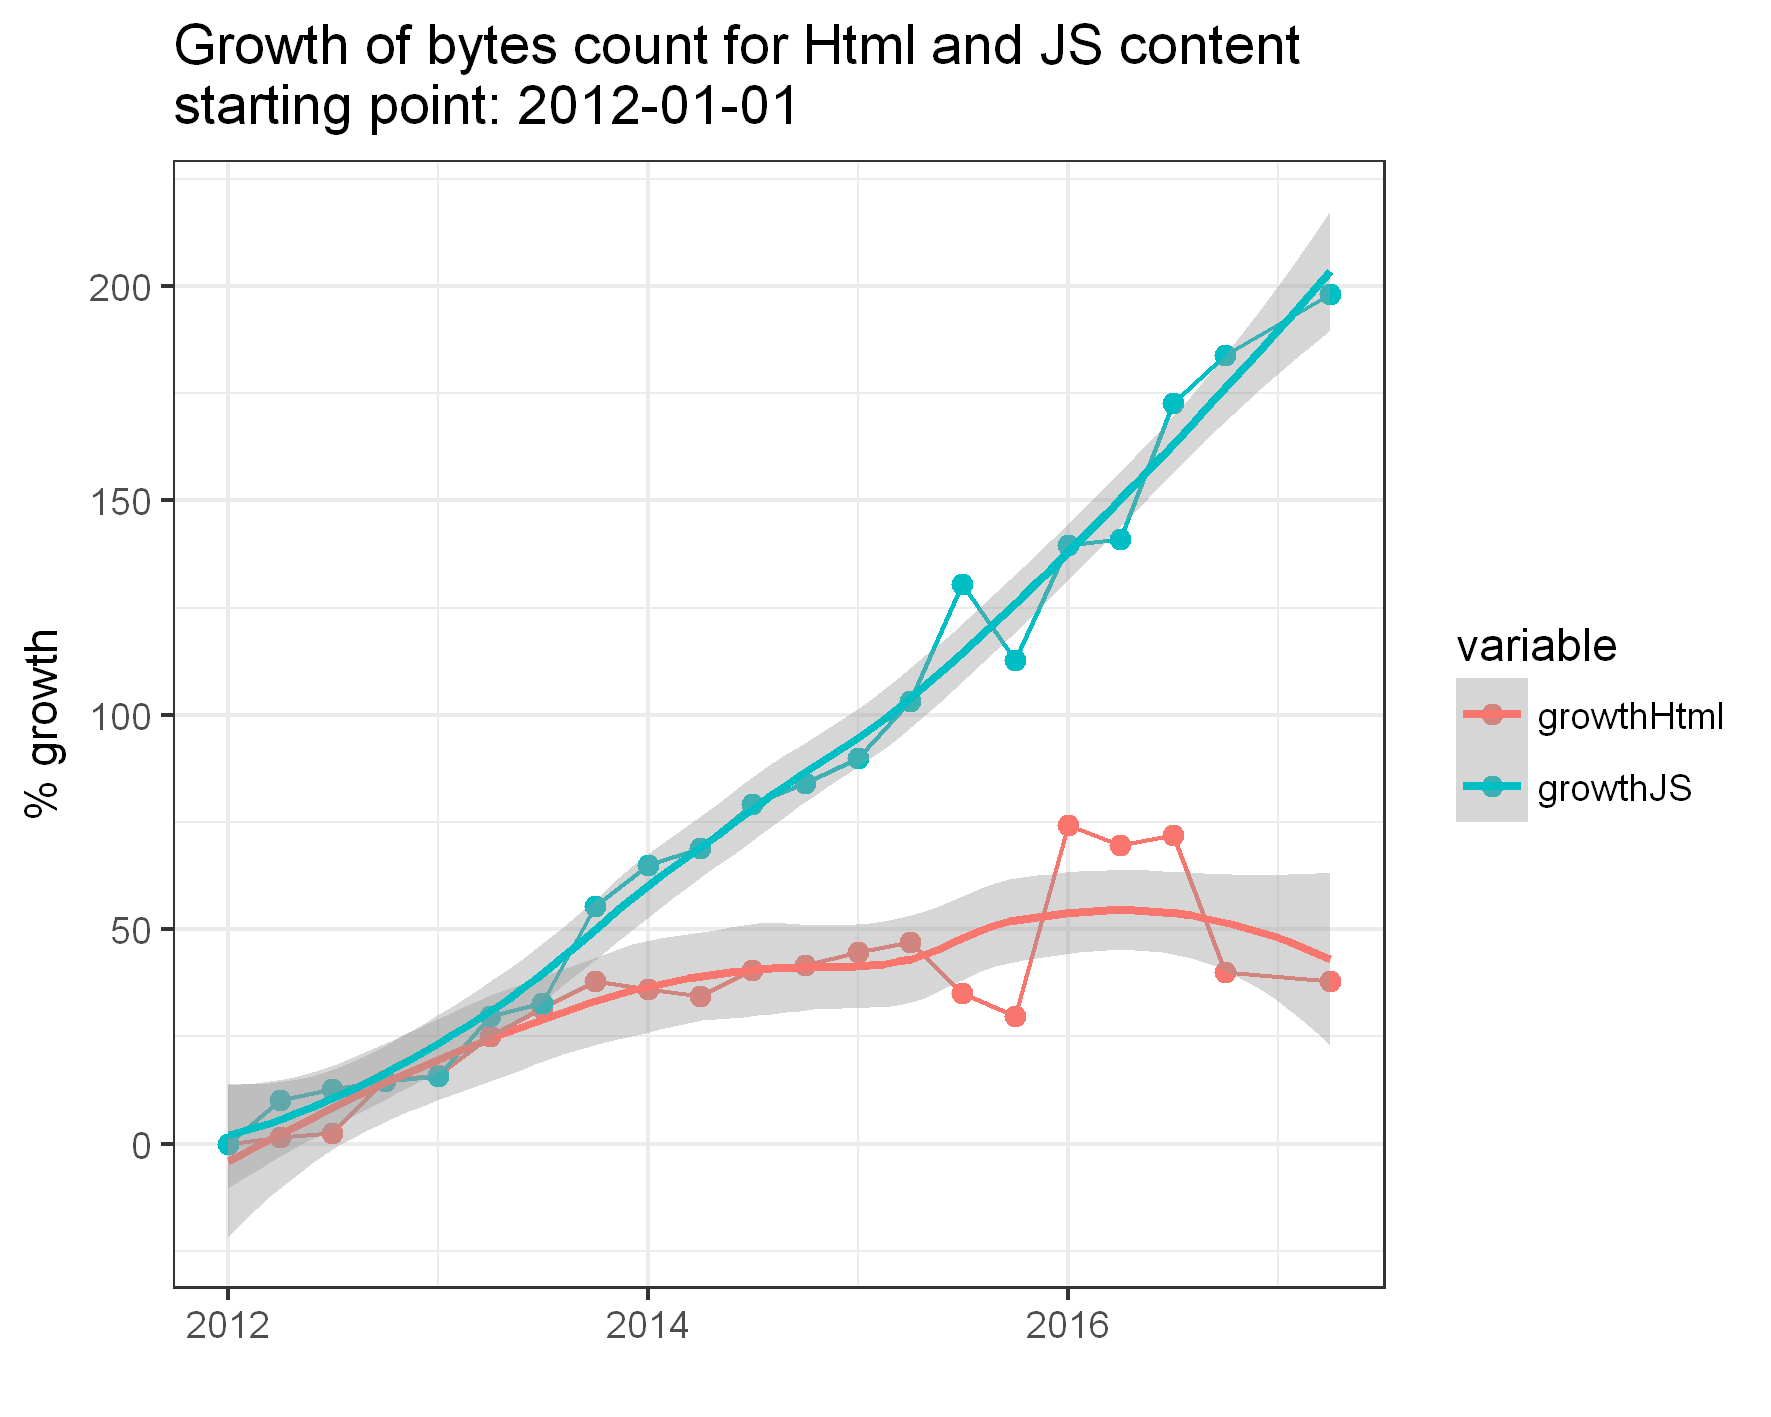
\includegraphics{../master/images/JSbytes.png}
\caption{JS bytes}
\end{figure}

\subsection{JS frameworks}\label{js-frameworks}

As for now the data about following frameworks was downloaded.

\begin{longtable}[]{@{}lllclc@{}}
\toprule
owner & name & date\_min & version\_first & date\_max &
version\_last\tabularnewline
\midrule
\endhead
angular & angular & 2015-03-14 & 0.0.1 & 2017-06-01 &
4.2.0\tabularnewline
jashkenas & backbone & 2010-10-13 & 0.1.0 & 2016-04-05 &
1.3.3\tabularnewline
webpack & webpack & 2013-12-19 & 1.0.0 & 2017-06-07 &
3.0.0\tabularnewline
nodejs & node & 2009-05-27 & 0.0.1 & 2017-06-06 & 8.0.0\tabularnewline
meteor & meteor & 2011-12-10 & 0.0.40 & 2017-06-06 & 1.6\tabularnewline
emberjs & ember.js & 2011-06-18 & 0.9 & 2017-05-31 &
2.14.0\tabularnewline
facebook & react & 2013-07-02 & 0.3.0 & 2017-05-01 &
15.5.4\tabularnewline
vuejs & vue & 2013-12-07 & 0.6.0 & 2017-05-09 & 2.3.3\tabularnewline
reactjs & redux & 2015-06-02 & 0.2.0 & 2016-09-04 & 3.6.0\tabularnewline
Polymer & polymer & 2013-07-11 & 0.0.20130711 & 2017-06-15 &
1.9.2\tabularnewline
\bottomrule
\end{longtable}

Some frameworks use only numeric versioning, while other use also
extended tags (e.g.~rc1, rc2, etc. - see
\protect\hyperlink{Versioning}{versioning}).

Some data was downloaded using
\href{https://developer.github.com/v4/}{GitHub GraphQL api}, some using
webscrapping techniques. For more details see R codes.

\subsubsection{NodeJS}\label{nodejs}

\begin{itemize}
\tightlist
\item
  \href{https://nodejs.org/}{Ofifcial webpage}
\item
  \href{https://en.wikipedia.org/wiki/Node.js}{Wikipedia}
\item
  \href{https://nodejs.org/en/about/releases/}{NodeJS releases policy}
\end{itemize}

Node.js is an open-source, cross-platform JavaScript run-time
environment for executing JavaScript code \textbf{server-side}.

Nodejs with its \href{https://github.com/nodejs/node/}{node repo} is
using number versioning, however they are releasing so often that in
description you have details about each release. Maybe in the future I
will extend the analysis with those details.

Last 10 releases:

\begin{longtable}[]{@{}lllll@{}}
\toprule
owner & name & date & version & version\_ext\tabularnewline
\midrule
\endhead
nodejs & node & 2017-06-06 & v6.11.0 & 6.11.0\tabularnewline
nodejs & node & 2017-05-30 & v8.0.0 & 8.0.0\tabularnewline
nodejs & node & 2017-05-03 & v7.10.0 & 7.10.0\tabularnewline
nodejs & node & 2017-05-02 & v6.10.3 & 6.10.3\tabularnewline
nodejs & node & 2017-05-02 & v4.8.3 & 4.8.3\tabularnewline
nodejs & node & 2017-04-11 & v7.9.0 & 7.9.0\tabularnewline
nodejs & node & 2017-04-04 & v4.8.2 & 4.8.2\tabularnewline
nodejs & node & 2017-04-04 & v6.10.2 & 6.10.2\tabularnewline
nodejs & node & 2017-03-29 & v7.8.0 & 7.8.0\tabularnewline
nodejs & node & 2017-03-21 & v7.7.4 & 7.7.4\tabularnewline
\bottomrule
\end{longtable}

\begin{verbatim}
<a href="https://plot.ly/~m.ziembinski/1/?share_key=BeYDrjyJ48pqdFRPOOJwlP" target="_blank" title="nodejs_releases" style="display: block; text-align: center;"><img src="https://plot.ly/~m.ziembinski/1.png?share_key=BeYDrjyJ48pqdFRPOOJwlP" alt="nodejs_releases" style="max-width: 100%;width: 600px;"  width="600" onerror="this.onerror=null;this.src='https://plot.ly/404.png';" /></a>

<script data-plotly="m.ziembinski:1" sharekey-plotly="BeYDrjyJ48pqdFRPOOJwlP" src="https://plot.ly/embed.js" async></script>
\end{verbatim}

\href{https://plot.ly/~m.ziembinski/1/}{Interactive chart}

\begin{verbatim}
<a href="https://plot.ly/~m.ziembinski/3/?share_key=NdcRn3bJqX3rP1q5Cqi6vo" target="_blank" title="nodejs_since" style="display: block; text-align: center;"><img src="https://plot.ly/~m.ziembinski/3.png?share_key=NdcRn3bJqX3rP1q5Cqi6vo" alt="nodejs_since" style="max-width: 100%;width: 600px;"  width="600" onerror="this.onerror=null;this.src='https://plot.ly/404.png';" /></a>

<script data-plotly="m.ziembinski:3" sharekey-plotly="NdcRn3bJqX3rP1q5Cqi6vo" src="https://plot.ly/embed.js" async></script>
\end{verbatim}

\href{https://plot.ly/~m.ziembinski/3/}{Interactive chart}

Other links: * \href{https://nodesource.com/node-by-numbers}{Node by
numbers}

\hypertarget{react}{\subsubsection{React}\label{react}}

\begin{itemize}
\tightlist
\item
  \href{https://facebook.github.io/react/}{Ofifcial webpage}
\item
  \href{https://en.wikipedia.org/wiki/React_(JavaScript_library)}{Wikipedia}
\end{itemize}

React is an open-source JavaScript library for \textbf{building user
interfaces}.

Facebook with its \href{https://github.com/facebook/react}{react repo}
is using mainly number versioning. After version v0.14.8 facebook change
the versioning and started with the version v15.0.0. See tables below:

Last 10 releases:

\begin{longtable}[]{@{}lllll@{}}
\toprule
owner & name & date & version & version\_ext\tabularnewline
\midrule
\endhead
facebook & react & 2017-05-01 & v15.5.1 & 15.5.1\tabularnewline
facebook & react & 2017-05-01 & v15.5.2 & 15.5.2\tabularnewline
facebook & react & 2017-05-01 & v15.5.3 & 15.5.3\tabularnewline
facebook & react & 2017-05-01 & v15.5.4 & 15.5.4\tabularnewline
facebook & react & 2017-04-07 & v15.5.0 & 15.5.0\tabularnewline
facebook & react & 2017-01-06 & v15.4.2 & 15.4.2\tabularnewline
facebook & react & 2016-11-23 & v15.4.1 & 15.4.1\tabularnewline
facebook & react & 2016-11-16 & v15.4.0 & 15.4.0\tabularnewline
facebook & react & 2016-09-19 & v15.3.2 & 15.3.2\tabularnewline
facebook & react & 2016-08-19 & v15.3.1 & 15.3.1\tabularnewline
\bottomrule
\end{longtable}

Major versions:

\begin{longtable}[]{@{}llrrlllll@{}}
\toprule
owner & name & major & N & date\_first & date\_last & previous &
since\_release & since\_previous\tabularnewline
\midrule
\endhead
facebook & react & 15 & 20 & 2016-03-08 & 2017-05-01 & 2015-07-03 & 419
days & 249 days\tabularnewline
facebook & react & 14 & 13 & 2015-07-03 & 2016-03-29 & 2015-02-22 & 270
days & 131 days\tabularnewline
facebook & react & 13 & 6 & 2015-02-22 & 2015-05-08 & 2014-10-16 & 75
days & 129 days\tabularnewline
facebook & react & 12 & 4 & 2014-10-16 & 2014-12-18 & 2014-07-13 & 63
days & 95 days\tabularnewline
facebook & react & 11 & 4 & 2014-07-13 & 2014-09-16 & 2014-03-19 & 65
days & 116 days\tabularnewline
facebook & react & 10 & 2 & 2014-03-19 & 2014-03-21 & 2014-02-17 & 2
days & 30 days\tabularnewline
facebook & react & 9 & 2 & 2014-02-17 & 2014-02-20 & 2013-12-19 & 3 days
& 60 days\tabularnewline
facebook & react & 8 & 1 & 2013-12-19 & 2013-12-19 & 2013-10-16 & 0 days
& 64 days\tabularnewline
facebook & react & 5 & 3 & 2013-10-16 & 2013-12-18 & 2013-07-17 & 63
days & 91 days\tabularnewline
facebook & react & 4 & 3 & 2013-07-17 & 2013-12-18 & 2013-05-29 & 154
days & 49 days\tabularnewline
facebook & react & 3 & 2 & 2013-05-29 & 2013-06-20 & NA & 22 days &
NA\tabularnewline
\bottomrule
\end{longtable}

\begin{verbatim}
<a href="https://plot.ly/~m.ziembinski/5/?share_key=FdzxOvNVE0chJmE5LnRCrl" target="_blank" title="react_releases" style="display: block; text-align: center;"><img src="https://plot.ly/~m.ziembinski/5.png?share_key=FdzxOvNVE0chJmE5LnRCrl" alt="react_releases" style="max-width: 100%;width: 600px;"  width="600" onerror="this.onerror=null;this.src='https://plot.ly/404.png';" /></a>
\end{verbatim}

\href{https://plot.ly/~m.ziembinski/5/}{Interactive chart}

\begin{verbatim}
<a href="https://plot.ly/~m.ziembinski/7/?share_key=5qKxdZdm86cIvgrnryTace" target="_blank" title="react_since" style="display: block; text-align: center;"><img src="https://plot.ly/~m.ziembinski/7.png?share_key=5qKxdZdm86cIvgrnryTace" alt="react_since" style="max-width: 100%;width: 600px;"  width="600" onerror="this.onerror=null;this.src='https://plot.ly/404.png';" /></a>
\end{verbatim}

\href{https://plot.ly/~m.ziembinski/7/}{Interactive chart}

NPM stats.

\begin{figure}
\centering
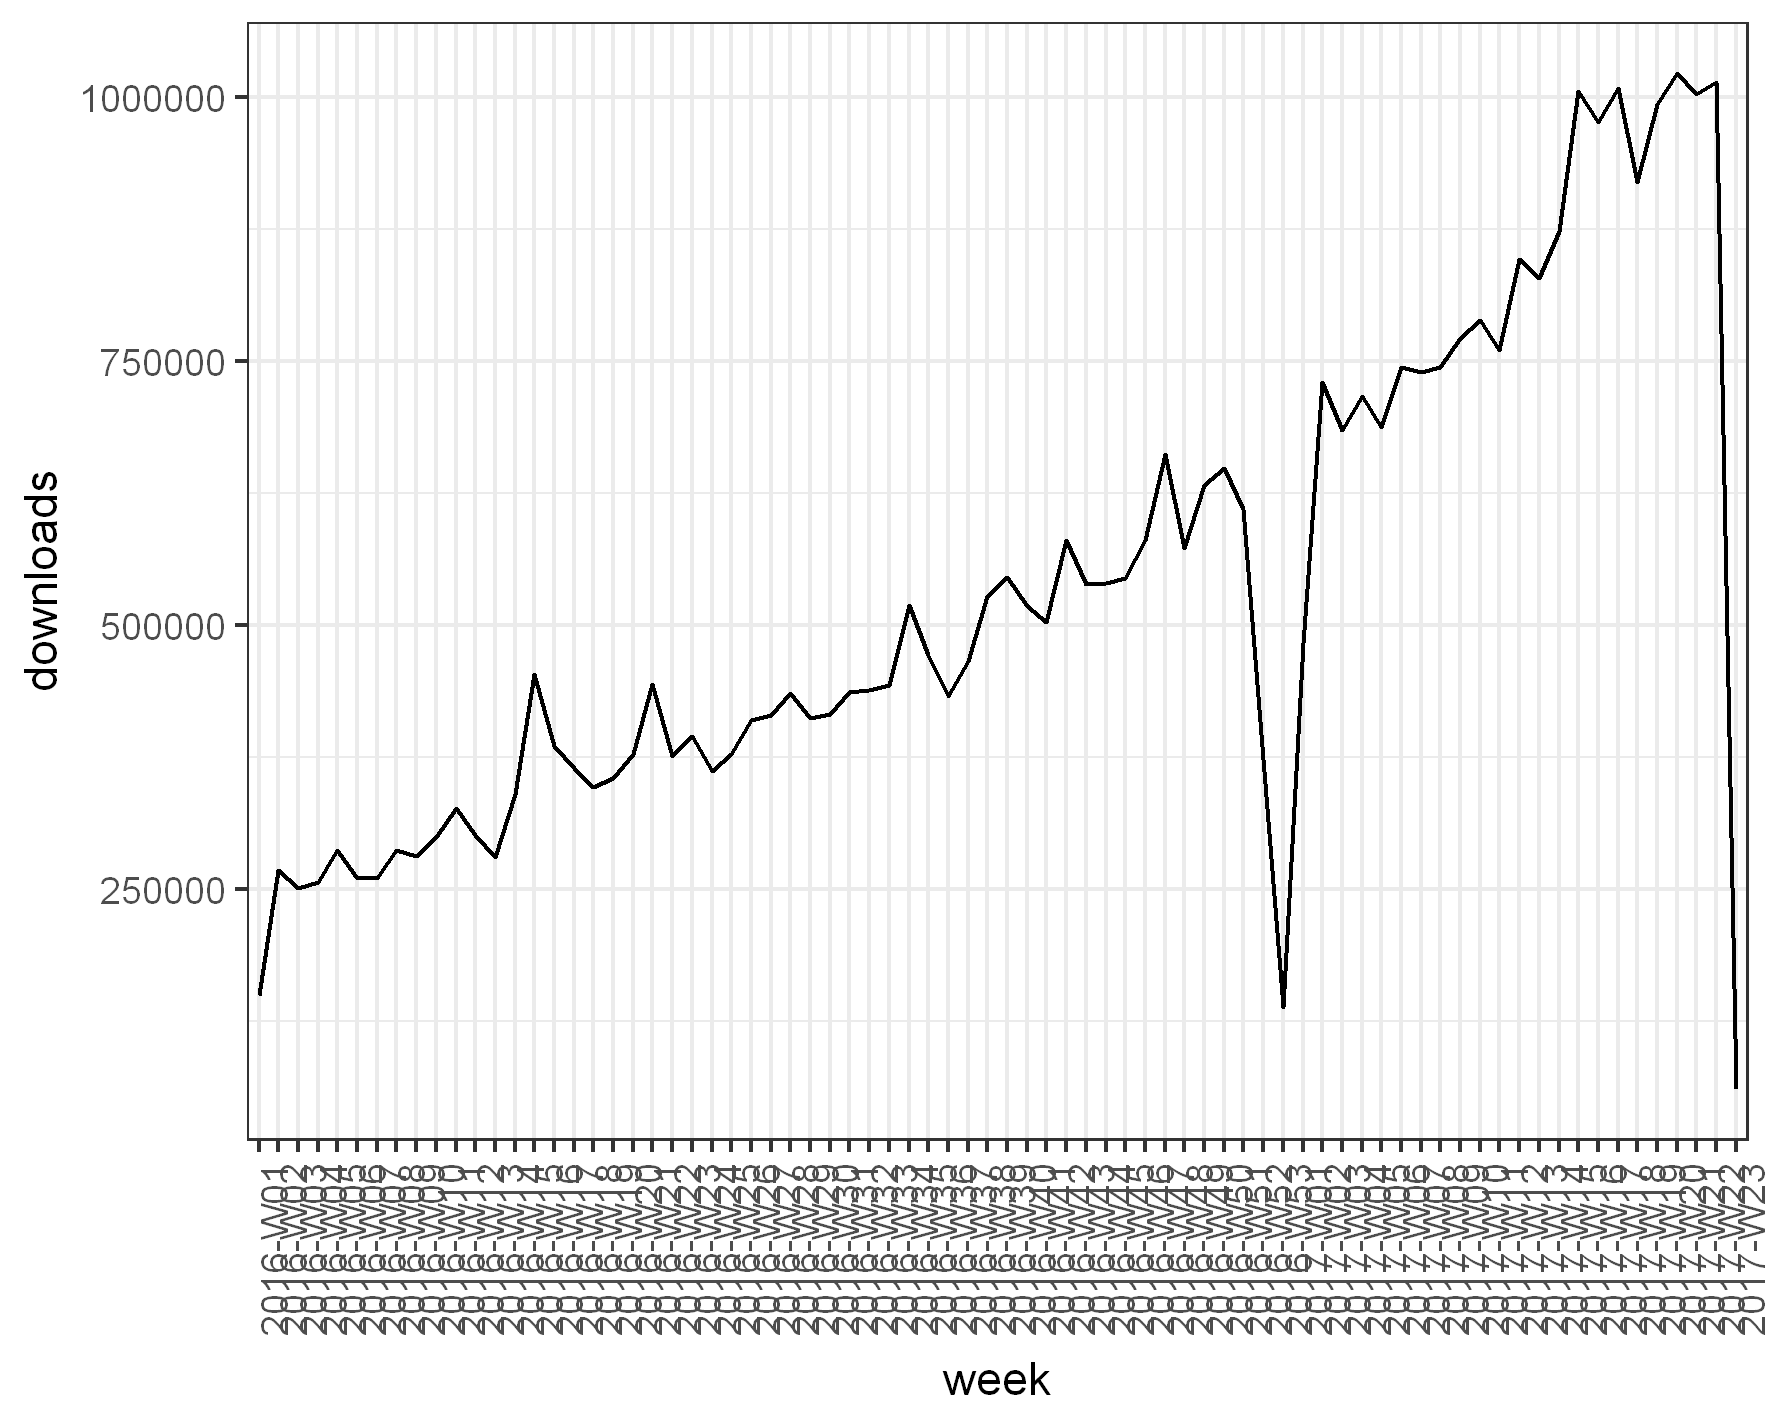
\includegraphics{../master/images/react_npm.png}
\caption{React npm stats}
\end{figure}

\subsubsection{Angular}\label{angular}

Last 10 releases:

\begin{longtable}[]{@{}lllll@{}}
\toprule
owner & name & date & version & version\_ext\tabularnewline
\midrule
\endhead
angular & angular & 2017-06-01 & 4.2.0-rc.2 & 4.2.0\tabularnewline
angular & angular & 2017-05-26 & 4.2.0-rc.1 & 4.2.0\tabularnewline
angular & angular & 2017-05-19 & 4.2.0-rc.0 & 4.2.0\tabularnewline
angular & angular & 2017-05-17 & 4.1.3 & 4.1.3\tabularnewline
angular & angular & 2017-05-10 & 4.2.0-beta.1 & 4.2.0\tabularnewline
angular & angular & 2017-05-10 & 4.1.2 & 4.1.2\tabularnewline
angular & angular & 2017-05-04 & 4.2.0-beta.0 & 4.2.0\tabularnewline
angular & angular & 2017-05-04 & 4.1.1 & 4.1.1\tabularnewline
angular & angular & 2017-04-26 & 4.1.0 & 4.1.0\tabularnewline
angular & angular & 2017-04-21 & 4.1.0-rc.0 & 4.1.0\tabularnewline
\bottomrule
\end{longtable}

Major versions:

\begin{longtable}[]{@{}llrrlllll@{}}
\toprule
owner & name & major & N & date\_first & date\_last & previous &
since\_release & since\_previous\tabularnewline
\midrule
\endhead
angular & angular & 4 & 30 & 2016-12-14 & 2017-06-01 & 2015-03-14 & 169
days & 641 days\tabularnewline
angular & angular & 2 & 113 & 2015-03-14 & 2017-03-17 & NA & 734 days &
NA\tabularnewline
\bottomrule
\end{longtable}

\href{https://plot.ly/~m.ziembinski/9/}{Interactive chart}

\subsubsection{Polymer}\label{polymer}

Last 10 releases:

\begin{longtable}[]{@{}lllll@{}}
\toprule
owner & name & date & version & version\_ext\tabularnewline
\midrule
\endhead
Polymer & polymer & 2017-06-15 & v1.9.2 & 1.9.2\tabularnewline
Polymer & polymer & 2017-06-15 & v1.9.2-dev & 1.9.2\tabularnewline
Polymer & polymer & 2017-05-25 & v2.0.1 & 2.0.1\tabularnewline
Polymer & polymer & 2017-05-15 & v2.0.0 & 2.0.0\tabularnewline
Polymer & polymer & 2017-05-13 & v2.0.0-rc.9 & 2.0.0\tabularnewline
Polymer & polymer & 2017-05-12 & v2.0.0-rc.8 & 2.0.0\tabularnewline
Polymer & polymer & 2017-04-19 & v2.0.0-rc.7 & 2.0.0\tabularnewline
Polymer & polymer & 2017-04-18 & v2.0.0-rc.6 & 2.0.0\tabularnewline
Polymer & polymer & 2017-04-17 & v1.9.1 & 1.9.1\tabularnewline
Polymer & polymer & 2017-04-17 & v1.9.1-dev & 1.9.1\tabularnewline
\bottomrule
\end{longtable}

Major versions:

\begin{longtable}[]{@{}llrrlllll@{}}
\toprule
owner & name & major & N & date\_first & date\_last & previous &
since\_release & since\_previous\tabularnewline
\midrule
\endhead
Polymer & polymer & 2 & 11 & 2017-03-04 & 2017-05-25 & 2015-05-27 & 82
days & 647 days\tabularnewline
Polymer & polymer & 1 & 45 & 2015-05-27 & 2017-06-15 & 2013-07-11 & 750
days & 685 days\tabularnewline
Polymer & polymer & 0 & 56 & 2013-07-11 & 2015-05-27 & NA & 685 days &
NA\tabularnewline
\bottomrule
\end{longtable}

\begin{verbatim}
<a href="https://plot.ly/~m.ziembinski/18/?share_key=fiPwZzAm4yedXtB24CxcnS" target="_blank" title="polymer_releases" style="display: block; text-align: center;"><img src="https://plot.ly/~m.ziembinski/18.png?share_key=fiPwZzAm4yedXtB24CxcnS" alt="polymer_releases" style="max-width: 100%;width: 600px;"  width="600" onerror="this.onerror=null;this.src='https://plot.ly/404.png';" /></a>
\end{verbatim}

\href{https://plot.ly/~m.ziembinski/18/}{Interactive chart}

\subsubsection{Redux}\label{redux}

Last 10 releases:

\begin{longtable}[]{@{}lllll@{}}
\toprule
owner & name & date & version & version\_ext\tabularnewline
\midrule
\endhead
reactjs & redux & 2016-09-04 & v3.6.0 & 3.6.0\tabularnewline
reactjs & redux & 2016-04-24 & v3.5.2 & 3.5.2\tabularnewline
reactjs & redux & 2016-04-20 & v3.5.0 & 3.5.0\tabularnewline
reactjs & redux & 2016-04-20 & v3.5.1 & 3.5.1\tabularnewline
reactjs & redux & 2016-04-08 & v3.4.0 & 3.4.0\tabularnewline
reactjs & redux & 2016-02-06 & v3.3.1 & 3.3.1\tabularnewline
reactjs & redux & 2016-02-05 & v3.3.0 & 3.3.0\tabularnewline
reactjs & redux & 2016-02-02 & v3.2.1 & 3.2.1\tabularnewline
reactjs & redux & 2016-02-01 & v3.2.0 & 3.2.0\tabularnewline
reactjs & redux & 2016-01-31 & v3.1.6 & 3.1.6\tabularnewline
\bottomrule
\end{longtable}

Major versions:

\begin{longtable}[]{@{}llrrlllll@{}}
\toprule
owner & name & major & N & date\_first & date\_last & previous &
since\_release & since\_previous\tabularnewline
\midrule
\endhead
reactjs & redux & 3 & 24 & 2015-09-12 & 2016-09-04 & 2015-09-01 & 358
days & 11 days\tabularnewline
reactjs & redux & 2 & 1 & 2015-09-01 & 2015-09-01 & 2015-06-30 & 0 days
& 63 days\tabularnewline
reactjs & redux & 1 & 4 & 2015-06-30 & 2015-08-15 & 2015-06-02 & 46 days
& 28 days\tabularnewline
reactjs & redux & 0 & 20 & 2015-06-02 & 2015-06-19 & NA & 17 days &
NA\tabularnewline
\bottomrule
\end{longtable}

\begin{verbatim}
<a href="https://plot.ly/~m.ziembinski/11/?share_key=AYm3iHj4wL2Rhs3zdM1Xim" target="_blank" title="redux_releases" style="display: block; text-align: center;"><img src="https://plot.ly/~m.ziembinski/11.png?share_key=AYm3iHj4wL2Rhs3zdM1Xim" alt="redux_releases" style="max-width: 100%;width: 600px;"  width="600" onerror="this.onerror=null;this.src='https://plot.ly/404.png';" /></a>
\end{verbatim}

\href{https://plot.ly/~m.ziembinski/11/}{Interactive chart}

\begin{verbatim}
<a href="https://plot.ly/~m.ziembinski/13/?share_key=l2jPV4Nh1kcH1nRxkcWvKo" target="_blank" title="redux_since" style="display: block; text-align: center;"><img src="https://plot.ly/~m.ziembinski/13.png?share_key=l2jPV4Nh1kcH1nRxkcWvKo" alt="redux_since" style="max-width: 100%;width: 600px;"  width="600" onerror="this.onerror=null;this.src='https://plot.ly/404.png';" /></a>
\end{verbatim}

\href{https://plot.ly/~m.ziembinski/13/}{Interactive chart}

\subsubsection{WebPack}\label{webpack}

Last 10 releases:

\begin{longtable}[]{@{}lllll@{}}
\toprule
owner & name & date & version & version\_ext\tabularnewline
\midrule
\endhead
webpack & webpack & 2017-06-07 & v3.0.0-rc.1 & 3.0.0\tabularnewline
webpack & webpack & 2017-06-05 & v3.0.0-rc.0 & 3.0.0\tabularnewline
webpack & webpack & 2017-05-25 & v2.6.1 & 2.6.1\tabularnewline
webpack & webpack & 2017-05-22 & v2.6.0 & 2.6.0\tabularnewline
webpack & webpack & 2017-05-06 & v2.5.1 & 2.5.1\tabularnewline
webpack & webpack & 2017-05-04 & v2.5.0 & 2.5.0\tabularnewline
webpack & webpack & 2017-04-14 & v2.4.1 & 2.4.1\tabularnewline
webpack & webpack & 2017-04-14 & v2.4.0 & 2.4.0\tabularnewline
webpack & webpack & 2017-04-13 & v1.15.0 & 1.15.0\tabularnewline
webpack & webpack & 2017-04-03 & v2.3.3 & 2.3.3\tabularnewline
\bottomrule
\end{longtable}

Major versions:

\begin{longtable}[]{@{}llrrlllll@{}}
\toprule
owner & name & major & N & date\_first & date\_last & previous &
since\_release & since\_previous\tabularnewline
\midrule
\endhead
webpack & webpack & 3 & 2 & 2017-06-05 & 2017-06-07 & 2015-11-01 & 2
days & 582 days\tabularnewline
webpack & webpack & 2 & 58 & 2015-11-01 & 2017-05-25 & 2013-12-19 & 571
days & 682 days\tabularnewline
webpack & webpack & 1 & 178 & 2013-12-19 & 2017-04-13 & NA & 1211 days &
NA\tabularnewline
\bottomrule
\end{longtable}

\begin{verbatim}
<a href="https://plot.ly/~m.ziembinski/15/?share_key=P6uelKPwQzB6KRXT71GMae" target="_blank" title="webpack_releases" style="display: block; text-align: center;"><img src="https://plot.ly/~m.ziembinski/15.png?share_key=P6uelKPwQzB6KRXT71GMae" alt="webpack_releases" style="max-width: 100%;width: 600px;"  width="600" onerror="this.onerror=null;this.src='https://plot.ly/404.png';" /></a>
\end{verbatim}

\href{https://plot.ly/~m.ziembinski/15/}{Interactive chart}

\begin{verbatim}
<a href="https://plot.ly/~m.ziembinski/17/?share_key=FeL9fpeCEZIjw660kA6NOX" target="_blank" title="webpack_since" style="display: block; text-align: center;"><img src="https://plot.ly/~m.ziembinski/17.png?share_key=FeL9fpeCEZIjw660kA6NOX" alt="webpack_since" style="max-width: 100%;width: 600px;"  width="600" onerror="this.onerror=null;this.src='https://plot.ly/404.png';" /></a>
\end{verbatim}

\href{https://plot.ly/~m.ziembinski/17/}{Interactive chart}

\subsubsection{Framework}\label{framework}

Last 10 releases:

Major versions:

\href{https://plot.ly/~m.ziembinski/5/}{Interactive chart}

\href{https://plot.ly/~m.ziembinski/7/}{Interactive chart}

\subsection{Appendix}\label{appendix}

\subsubsection{Something about JS}\label{something-about-js}

\begin{itemize}
\tightlist
\item
  \href{https://medium.com/@bojzi/overview-of-the-javascript-ecosystem-8ec4a0b7a7be}{Overview
  of the JavaScript ecosystem}
\item
  \href{https://www.imaginarycloud.com/blog/a-javascript-ecosystem-overview/}{A
  JAVASCRIPT ECOSYSTEM OVERVIEW}
\item
  \href{https://medium.com/@ericclemmons/javascript-fatigue-48d4011b6fc4}{JavaScript
  Fatigue}
\item
  \href{http://www.confluentforms.com/2016/01/javascript-churn-technology-investment-effect.html}{The
  current JavaScript churn, and its long-term effect on your business}
\end{itemize}

\subsubsection{Other useful links if you want to know how Internet is
working}\label{other-useful-links-if-you-want-to-know-how-internet-is-working}

\begin{itemize}
\tightlist
\item
  \href{https://npm-stat.com/}{npm statistics}
\item
  \href{https://builtwith.com/}{Find out what websites are Built With}
\item
  \href{http://libscore.com/}{Libscore - stats on JavaScript library
  usage}
\item
  \href{http://stateofjs.com/}{the State of JavaScript Survey}
\end{itemize}

\subsubsection{Versioning}\label{versioning}

I won't go into details of the details of a software release life cycle,
as they can be easily check, e.g on
\href{https://en.wikipedia.org/wiki/Software_release_life_cycle}{Wikipedia}.
Here you can find meanings of the most common abbreviations:

\begin{itemize}
\tightlist
\item
  GA - General availability (a release); should be very stable and
  feature complete
\item
  RC - Release candidate; probably feature complete and should be pretty
  stable - problems should be relatively rare and minor, but worth
  reporting to try to get them fixed for release.
\item
  M - Milestone build - probably not feature complete; should be vaguely
  stable (i.e.~it's more than just a nightly snapshot) but may still
  have problems.
\item
  LTS - Long-term support; a type of special versions or editions of
  software designed to be supported for a longer than normal period.
\end{itemize}

\begin{figure}
\centering
\includegraphics{https://i.stack.imgur.com/UP0W0.pnga}
\caption{software release life cycle}
\end{figure}

\subsubsection{Awesome GraphQL}\label{awesome-graphql}

\begin{itemize}
\tightlist
\item
  \href{https://github.com/chentsulin/awesome-graphql}{awesome-graphql}
\item
  \href{https://github.com/APIs-guru/graphql-apis}{APIs-guru}
\end{itemize}

\subsubsection{To Do}\label{to-do}

\begin{itemize}
\tightlist
\item
  analysis of alpha, beta and rc releases
\item
  summary of all frameworks releases
\item
  github pages webpage to present data
\item
  why release dates are different in graphql database and tags web?
  \textgreater{} diff between releases and tags. React data suggest that
  tag dates are better (see react ver. 0.10-0.12).
\item
  download other libriaries
\item
  changing charts to d3 to consider
\end{itemize}

\subsubsection{Notes}\label{notes}

pandoc -r markdown -w latex -o latex/outfile.tex README.md
